

\section{Conception et développement de modèle}

La prédiction du prix d'une action ou son rendement par une série temporelle financière fait l'objet de nombreuse recherches. Pour atteindre notre objectif, nous avons proposé le modèle de réseaux de neurones pour faire la prédiction. L’entrée et la sortie de notre projet sont très différentes par rapport aux autres projets. Les entrées sont les 13 TIs, comme nous le savons, avoir plus de TIs permet d'obtenir plus d’informations, mais il y a aussi plus de risques d’avoir trop de redondances en prenant plusieurs TIs de la même catégorie. La sortie est le rendement à un horizon prédefini, il est plus difficile de prédire la vraie valeur que la tendance (mettre une seuil comme signal d’achat ou de vente). Dans cette partie, nous présentons la façon de construction de la base d'apprentissage, le pré-traitement sur les données d'origines et les paramètres de la base d'apprentissage. 

\subsection{Construction de la base d’apprentissage}

La base d'apprentissage en entrée du réseau de neurones est composée de patterns, et chaque pattern représente les données d'un jour, qui contient 13 TIs : 5 TIs qui indiquent la tendance du marché, 3 TIs qui représentent l'ampleur, 3 TIs qui expriment la volatilité et 2 TIs qui symbolisent le volume. Comme notre modèle d'apprentissage de la prédiction du rendement est supervisé, nous avons besoin d’ajouter les labels pour les patterns correspondants, c’est-à-dire qu'il faut calculer le rendement à un certain horizon pour chaque pattern. La formule permettant de calculer le rendement est $ r = \frac{P_{t_{0}+h_{0}}}{P_{t_{0}}} - 1 $.


\subsubsection{Pré-traitement de données}

Les données de 13 TIs sont sur des échelles différentes. Dans un premier temps, nous avons utilisé directement ces données calculées, parce que nous avions supposé que notre modèle de réseau de neurones est capable de s'adapter pour les normaliser, cela signifie que les grandes valeurs ne vont pas être considérées comme plus importantes que les petites. Cependant, quand nous avons fait le premier test sur ces données, nous avons eu un résultat qui n’était pas idéal. Le réseau de neurones n'a pas réussi à apprendre l'évolution de la courbe de rendement et la prédcition est loin d'être bonne. Ensuite, nous avons normalisé ces entrées en utilisant la formule $\frac{V-V_{min}}{V_{max}-V_{min}}$, ainsi les valeus de 13 TIs ont été ramenées dans une fourchette de [0,1]. Dans ce cas, le poids attribué à chaque TI dont le réseau tient compte est correct. Après avoir appliqué la normalisation, le résultat est meilleur et la valeur de prédiction s'est approchée vers la vraie valeur.

\subsubsection{Paramétrage de la base d'apprentissage}

Pour notre projet, il faut aussi faire varier les paramètres différents pour construire la base d'apprentissage, qui sert à tester des différents scénarios. Nous prenons principalement 4 paramètres pour comparer le résultat de chaque scénario : l'horizon, la taille d'apprentissage, la durée du test et le nombre de TI. Pour lancer des tests sur les différents scénarios, nous faisons chaque fois varier seulement un paramètre afin de trouver la meilleure combinaison de paramètres.\\

Nous avons pris tous les 13 TIs au début de notre projet, nous voudrons collecter plus d’informations pour faire la prédiction, nous avons considéré que cette combinaison de TIs est plus robuste. Pour savoir si le nombre de TIs a un impact sur la performance de notre système, nous avons diminué le nombre de TIs et refait des tests avec la dimension réduite en entrée du réseau. Les nombres de TIs que nous avons choisi sont 13, 12 (élimination d'un TI aléatoire) et 4 (un TI par catégorie).

   	
\subsection{Choix du modèle}

De nombreuses études ont largement admis que la non-linéarité existe sur les marchés financiers et que les réseaux de neurones peuvent être efficacement utilisés pour découvrir cette relation. Les modèles de réseaux de neurones pour l'estimation sont ensuite examinés pour leur capacité à fournir une prévision efficace des valeurs futures.\\

Nous avons utilisé l'algorithme de perceptron multicouche à rétropropagation. Le perceptron multicouche est un type de réseau organisé par plusieurs couches, chaque couche est constituée d'un nombre variable de neurones, les neurones de la dernière couche étant les sorties du système global. Dans notre cas, l'entré de reseau est les TIs et la sortie est le rendement. L'algoritnme de rétropropagation du gradient déscendant est pour minimiser l'erreur afin de converger. La figure \ref{fig:RN} représente la structure de notre réseau de neurones :

\begin{figure}[H]
\centering
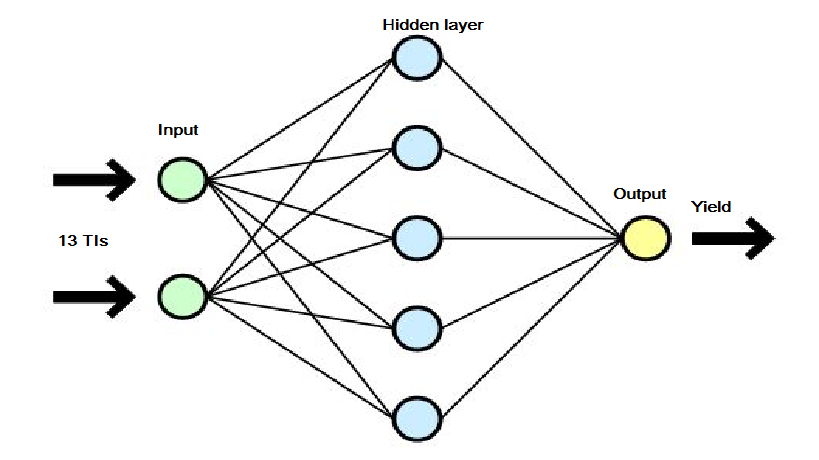
\includegraphics[width=.9\linewidth, scale=0.2]
{plot/RN.png}
\caption{Le schéma du réseau de neurones}
\label{fig:RN}
\end{figure}

Pour être plus clair, nous présentons les patterns d'entrée en format matriciel : 

\begin{figure}[H]
\centering
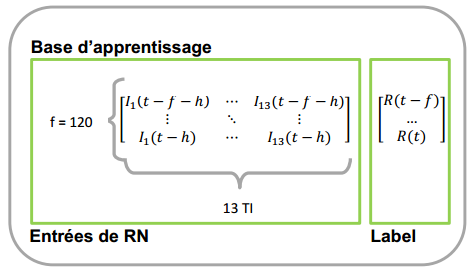
\includegraphics[width=.9\linewidth, scale=0.2]
{plot/base.png}
\caption{L'entrée de base d'apprentissage}
\label{fig:base}
\end{figure}


\subsection{Préparation des scénarios}





